% !TEX root = MasterPaper.tex
\chapter{先行研究}
\thispagestyle{fancy} % このページのみ
\lhead{}
\chead{}
\rhead{}
\lfoot{} 
\cfoot{\thepage}  
\rfoot{}
%

\section{遺伝的アルゴリズム}
\label{sec2.1}

\subsection{遺伝的アルゴリズムの概要}
\label{sec2.1.1}

GAとは選択淘汰や突然変異など生物進化の仕組みを模範した最適化アルゴリズムである.GAは1975年にJ.H.Hollandnによって提案された手法である.GAの枠組みはとても簡単であり,与えられた最適化問題の評価関数に対して,いくつかの乱数と単純な記号処理を用いるだけで求めることができる.また,GAは他の最適化アルゴリズムより比較的少ない計算量で最適解を求めることができる.

GAのフローチャートを図2.1に示す.GAでは,生成した遺伝子列に対して,選択,交叉,突然変異といった生物進化の仕組みを模した処理を行う.問題の解候補を生物集団の各個体と呼び,各個体のパラメータを遺伝子と呼ぶ.

以下に図2.1の具体的な流れについて述べる.


\begin{description}
\item[ (1) ]遺伝子型の決定

GAの対象となる問題を遺伝子列に変換する.

\item[ (2) ]初期遺伝子集団の決定

(1)で決められた遺伝子型で,要素の異なるさまざまな個体をランダムに発生させる.

\item[ (3) ]適応度評価

生成された遺伝子集団に対して評価を行い,各個体の適応度をあらかじめ定められた計算方法と評価で算出する.

\item[ (4) ]選択処理

遺伝子集団中における各個体の適応度に基づいて,交叉処理を行う個体を選択する.

\item[ (5) ]交叉処理

(4)で選択された2つの個体間で遺伝子を組み替えて新しい個体を発生させる.

\item[ (6) ]突然変異処理

遺伝子のある部分を特定の確率で強制的に変化させる.

\item[ (7) ]終了条件(遺伝子集団の評価)

生成された次世代の遺伝子集団が,GA処理を終了するための評価基準を満足しているかどうかを確認する.
\end{description}

\begin{figure}[p]
\begin{center}

\vspace{1.5cm}
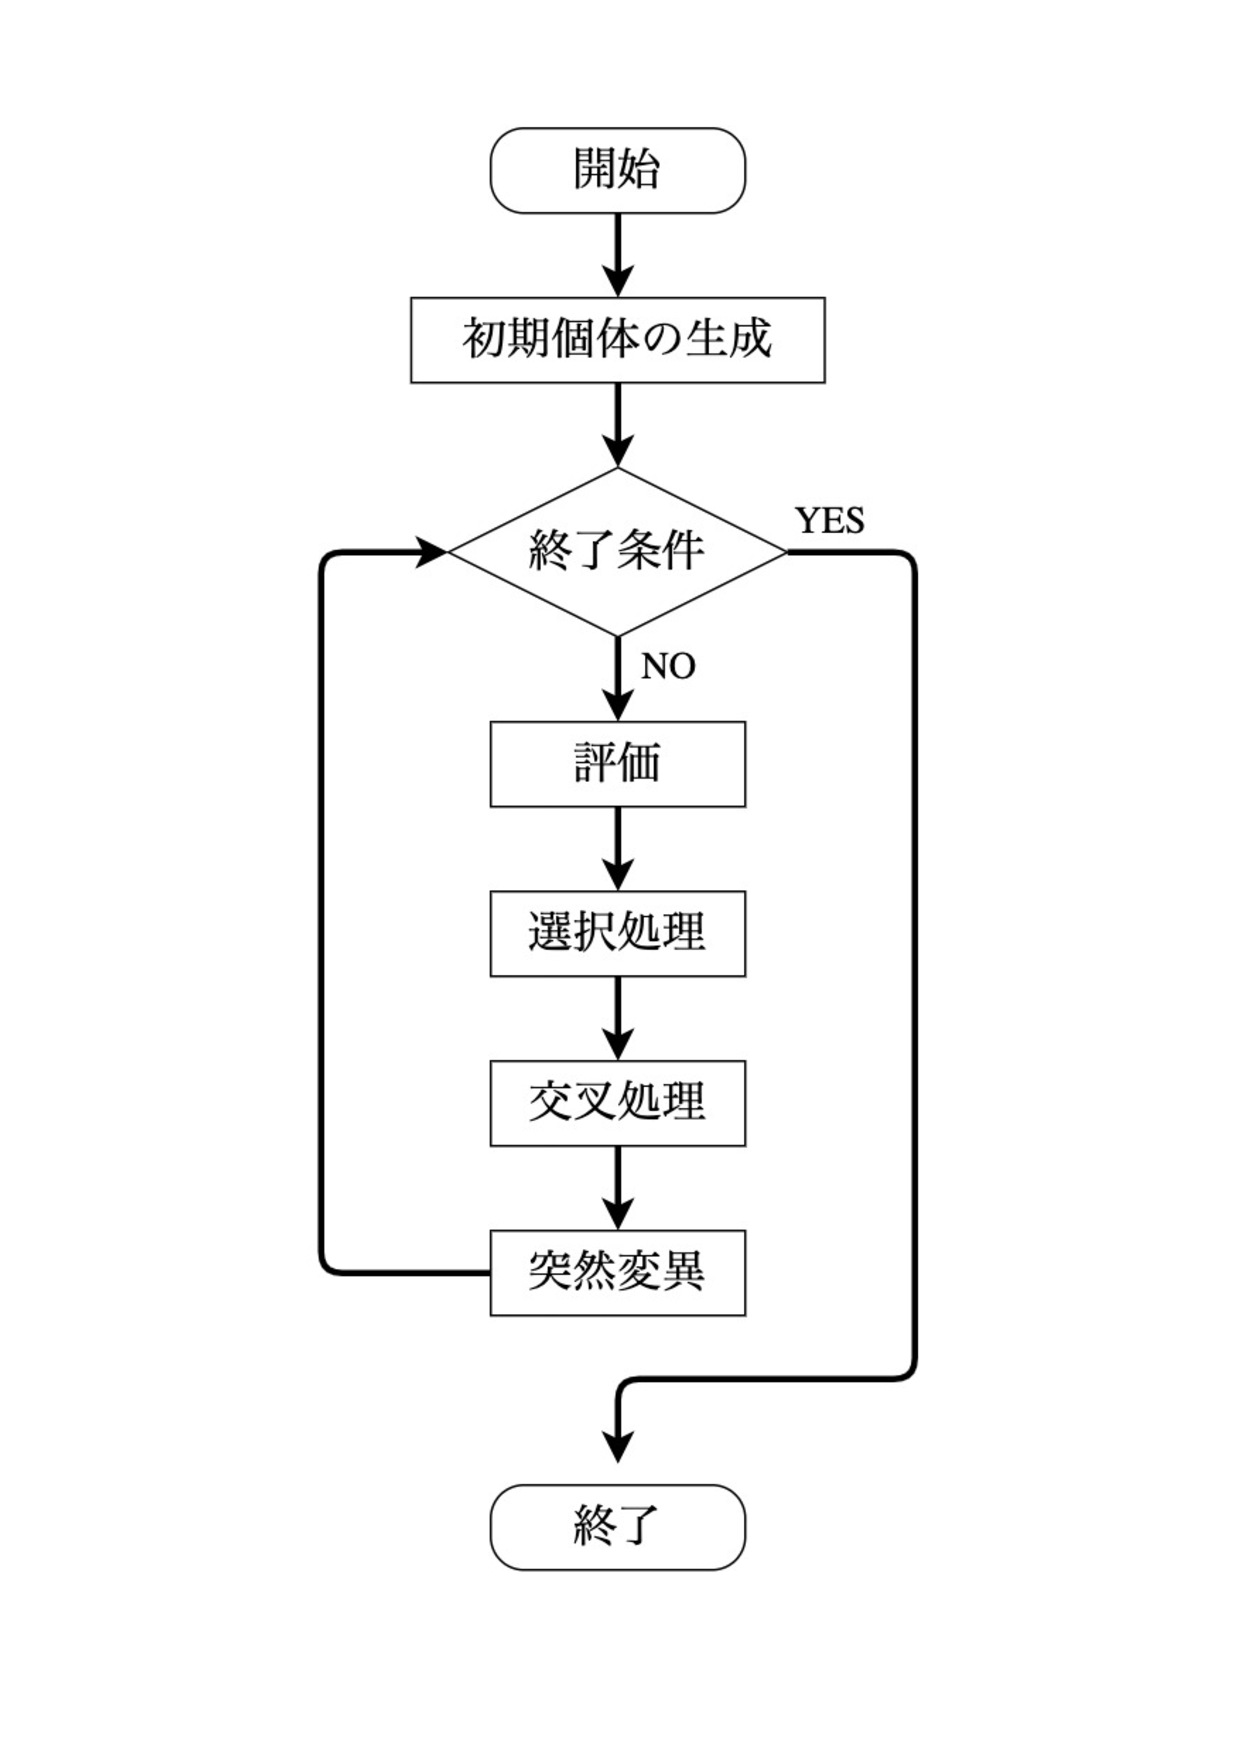
\includegraphics[scale=0.75]{figurefolder/chapter2/GaFlowchart.pdf}
\caption{遺伝的アルゴリズムのフローチャート}
\label{遺伝的アルゴリズムのフローチャート}

\end{center}
\end{figure}

\clearpage


\subsection{各個体の評価処理}
\label{sec2.1.2}
  
各個体の評価処理は,あらかじめ定めた適応度により,各個体の適応度を求める操作である.本処理は遺伝子型と設定されている記号列を実際の評価型にデコーディングして,その表現型と設定されている環境との適応を判定することによって行われる.個体間の適応度の差が激しい場合,選択処理時に適応度の高い個体が選ばれる確率が非常に高くなる.その個体の遺伝子が集団内に増加することにより短時間で探索が収束してしまうため,より適応度の高い遺伝子の探索が困難となる.そこで,適応度の値を直接反映させるのではなく,関数を用いて変換してから,選択に反映させるスケーリングを行う.スケーリング関数の例を示す.表2.1において$f$は元の適応度,$f'$は新たな適応度である.べき乗スケーリングにおいて,$k$はスケーリング指数と呼ばれる.また,シグマ切断の関数において,$\sigma$は適応度の標準偏差,$\bar{f}$は適応度の平均値である.



\begin{table}[!ht]
\caption{スケーリング関数の例}
\label{tb:sk}
\begin{center}
\begin{tabular}{|c||c|}\hline
スケーリング & 関数 \\ \hline
線形スケーリング & $f'=af+b$ \\ \hline
べき乗スケーリング & $f'=f^{k}$ \\ \hline
シグマ切断 & $f'=f-( \bar{f} - c \times \sigma )$ \\ \hline
\end{tabular}
\end{center}
\end{table}

\newpage


\subsection{選択処理}
\label{sec2.1.3}

各個体の選択処理は,集団内での適応度の分布にしたがって,交叉を行う個体の生存分布を決定する操作である.以下に,基本的な選択処理方法である適応度比例方式とエリート保存方式について述べる.

\begin{description}
\item[ (1) ]適応度比例方式

適応度比例方式はルーレット選択方式とも呼ばれ,各個体の子孫がその適応度に比例した確率で選択される方法である.適応度比例方式の最も簡単な実現方法は,適応度に基づいた円グラフをルーレットとして回し,ルーレットの玉が入った領域の個体を選び出すというものである.式(\ref{eq:2.1})に重み付けルーレット方式の式を示す.



\begin{equation}
\vspace{1.0cm}
{p_i}=\frac{f_i}{\displaystyle\sum_{i=1}^{n}f_i}
\label{eq:2.1}
\vspace{-0.5cm}
\end{equation}
式(\ref{eq:2.1})において,$p_i$は$i$番目の個体が親として選ばれる確率,$f_i$は$i$番目の個体適応度,$n$は個体数である.

\item[ (2) ]エリート保存方式

エリート保存方式は,個体の中で最も適応度の高い個体はそのまま次世代に残すという方法である.最も適応度の高い個体は交叉や突然変異による変形を受けないという利点がある.ただし場合によってはあまり良くない遺伝子が急速に集団中に広がる.つまり局所的最適解に収束する危険性がある.そのため一般的には他の選択方法と組み合わせて用いられる.

\end{description}

\newpage

\subsection{交叉処理}
\label{sec2.1.4}

交叉処理は,2つの染色体間で,遺伝子を組み替えて,新たな個体を発生させる操作である.交叉処理で用いられる基本的な手法である一点交叉,複数点交叉,一様交叉について遺伝子列がビット列である場合の例を図に示す.



\begin{description}
\item[ (1) ]一点交叉

図に示すように,遺伝子上に交叉位置をランダムで一点決定する.交叉位置で,親1と親2の遺伝子を入れ替え,子1と子2を発生させる.


\item[ (2) ]複数点交叉

図に示すように,遺伝子上に複数の交叉位置を作る.交叉位置ごとに親1と親2の遺伝子を入れ替え,子1と子2を発生させる.

\item[ (3) ]一様交叉

図に示すように,マスクパターンをランダムに生成する.そして,2つの親個体に対し,そのマスクのビットが0であるなら親1を,1であるなら親2の遺伝子をコピーして子1を発生させる.同時に逆のコピーを行い,子2を発生させる.

\end{description}

\newpage

\begin{figure}[p]
\begin{center}


\subfigure[一点交叉]{
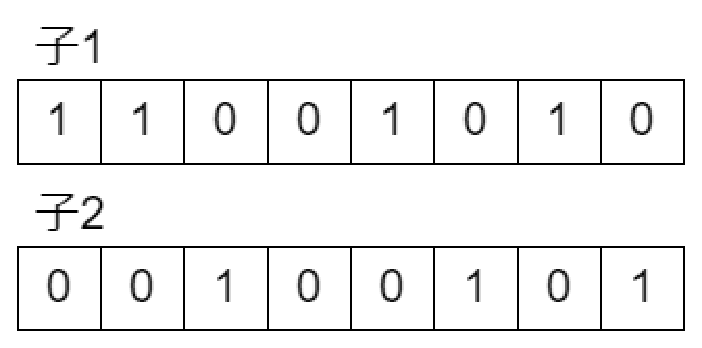
\includegraphics[width=15cm]{figure/chapter2/mikawa2.eps}
\label{一点交叉}}

\subfigure[複数点交叉]{
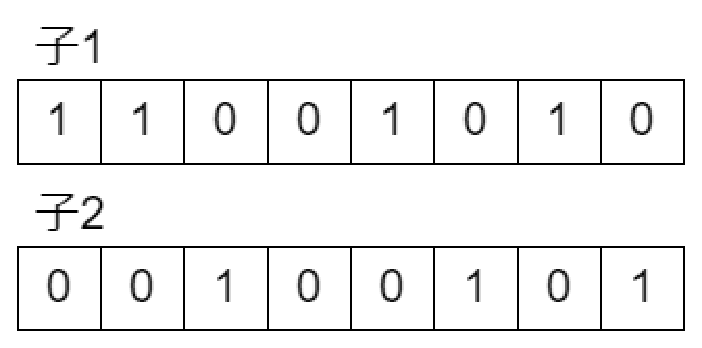
\includegraphics[width=15cm]{figure/chapter2/mikawa2.eps}
\label{複数点交叉}}

\subfigure[一様交叉]{
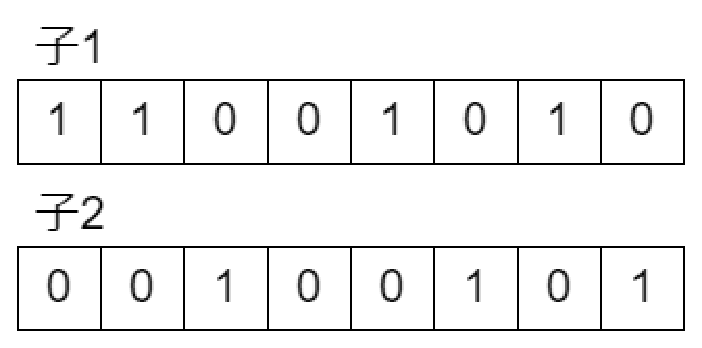
\includegraphics[width=15cm]{figure/chapter2/mikawa2.eps}
\label{一様交叉}}

\caption{交叉処理}
\label{tb:cross}


\end{center}

\end{figure}



\clearpage



\subsection{突然変異処理}
\label{sec2.1.5}

突然変異処理は,遺伝子のある部分を特定の確率で強制的に変化させる操作である.この操作により遺伝子集団に多様性をもたせることでより良い解を持つ個体の発生を促す.ただし,突然変異の確率を大きくしすぎると解の収束が遅くなる.

\begin{description}

\item[ (1) ]転座方式

図に転座方式を示す.転座方式は,遺伝子の一部が同じ遺伝子の他の部分,または他の遺伝子上に位置を移す処理である.

\item[ (2) ]逆位方式


図に逆位方式を示す.逆位方式は,部分的に遺伝子の配列順序を入れ替える処理である.


\end{description}


\newpage

\section{対話型進化計算}
\label{sec2.2}

\subsection{対話型進化計算の概要}
\label{sec2.2.1}

感性情報を扱うまでは情報処理におけるシステムの最適化は,望ましい出力パラメータを調節することであった.ほとんどの場合,システムの望ましい出力は定量的なものであり,主に誤差最小化規範などを代表とする各種最適化手法が開発されてきた.

しかし近年では,情報処理におけるシステムの最適化の対象は感性情報にまで及んでいる.その場合,望ましい出力がユーザが好む音楽や画像などユーザ自身が主観的に決めるものであるため,望ましい出力を数値的に導くことは困難である.このようなシステムの最適化において,従来と異なる最適化手法が必要となる.その方法の一つとして,ユーザの評価系の代替モデルを作成し,これを従来の最適化システムに組み込むことで数値的に導き出せるようにすることが考えられる.しかし,個人の主観や好みに依存する情報に対応できる正確な代替モデルを構築することは非常に難しい.そこで,ユーザ自身が最適化系に組み込み,ユーザ本人の評価に基づいてコンピュータに最適化させる方法が考えられる.このようにユーザとコンピュータがコミュニケーションをとり,ユーザの主観的評価に基づいて最適化を行う手法のうち,ECを用いる手法をIECと呼ぶ.IECは人間の主観的評価に基づいて最適化を行うため,感性を具現化する技術といえる.

代表的なEC 技術として,GA,タブーサーチ法(Taboo Serch: TS),遺伝的プログラミング (Genetic Programming: GP),進化戦略 (Evolution Strategy: ES),進化的プログラミング (Evolutionary Programming: EP),粒子群最適化 (Particle Swarm Optimization: PSO) などがある.
    
\subsection{対話型遺伝的アルゴリズム}
\label{sec2.2.2}

本研究では,GAにおける評価系に人の感性を組み込んだ手法であるIGAを用いる.
IGAは,GA処理における解候補評価をユーザが自らの感性に基づいて行い,解候補を最適化する手法である.

IGAの基本的な処理の流れを図に示す.まず初期解候補を生成する.次に,解候補をユーザに提示し,ユーザが主観的評価を行う.ユーザによる評価が終了すると,ユーザによって与えられた各解候補の評価をもとに選択・交叉・突然変異等の処理が行われ,新たな解候補を生成し,再びユーザに提示する.このような処理を繰り返し,ユーザの感性に合う解候補を生成する.

IGAは,ユーザ評価を取り入れた進化計算手法であるIECにおいてGAの進化計算アルゴリズムを適応させた手法である.すなわち,IGAとは通常のGAにおいて適応度を決定する処理をユーザが行う手法である.ユーザの主観的評価が適応度に反映されるため,IGAは特にユーザの感覚的,直観的な評価が必要とされる問題の解決に多く用いられる.また一般的にIGAはユーザの評価回数が多いほど最適化性能が高くなる傾向にある.したがって,IGAを用いた最適化システムが十分な最適化性能を発揮するためには多くのユーザ評価が必要となる.しかし,ユーザに多くの評価を求めることは,ユーザの評価負担の増加に繋がる可能性がある.



\newpage

\section{感性とロボット}
\label{sec2.3}

\subsection{ロボットの進化}
\label{sec2.3.1}
近年,ロボット技術の進歩は著しい.人間の代わりに工場などで様々な作業の自動化を行う産業用ロボットは.1960年代に初めて実用化され,普及し始めた.この時代のロボットは,ただ同じ作業を繰り返すだけの作業の代替をするだけであったが,ロボット技術の進歩により様々なロボットが登場した.ロボットはAI,センサ,アームなどの技術進歩によって従来よりも複雑な作業をこなせるようになった.従来の産業用ロボットは比較的大型であり,人との協働作業には不向きであったが,近年では人と協働作業をすることを前提として開発された協働ロボットが実用化されている.
現在では産業用ロボットだけでなく,非産業ロボットであるサービスロボットが普及している.サービスロボットには医療用ロボット,案内ロボット,コミュニケーションロボットなどがある.コミュニケーションロボットには認知所の予防や癒し効果などが期待でき,今後普及が進むと予想されている.


\subsection{性格特性とハンドジェスチャ}
\label{sec2.3.2}
人間らしいコミュニケーションロボットを実現するためには,ロボットの性格特性をジェスチャなどを用いて表現することが重要であるとされている[][].ハンドジェスチャには言葉を強調したり,意味を補完する効果がある[].個人の性格を測る指標としてBig-5理論がよく用いられる.Big-5理論とは,心理学における人の性格は突き詰めると5つの要素の組み合わせからなるとした理論である.Big-5理論における性格特性は,「Openness(開放性)」,「Conscientiousness(誠実性)」,「Extraversion(外向性)」,「Agreauleness(協調性)」,「Neuroticism(神経症的傾向)」から構成される.
Big-5理論は心理学のみならず様々な分野で活用されている.対話中の動作から性格特性を推測する研究[][]や,性格特性からエージェントジェスチャを生成する研究[]などがある.性格特性とハンドジェスチャに関して多くの先行研究がある.ハンドジェスチャは性格特性を表現する重要な指標であることが示されている[][][].
また,性格特性を構成する要素である外向性とハンドジェスチャの関連性について特に多くの研究がされており,外向性の値とハンドジェスチャのスピードや大きさが正の相関があることが示されている[].
また,外向性の値とハンドジェスチャの表出頻度も正の相関があることが示されている[].






\vspace{1cm}
\begin{figure}[!h]
 \begin{center}
  \centering
  \label{fig:kansei}
 \end{center}
\end{figure}

